%%%%%%%%%%%%%%%%%%%%%%%%%%%%%%%%%%%%%%%%%%%%%%%%%%%%%%%%%%%%%%%%%%%%%
%
% talk intro optimization Cotonou 2022
%
%%%%%%%%%%%%%%%%%%%%%%%%%%%%%%%%%%%%%%%%%%%%%%%%%%%%%%%%%%%%%%%%%%%%%

\documentclass[12pt]{beamer}
\usepackage[utf8]{inputenc}
\usepackage{amsmath}
\usepackage{amsfonts}
\usepackage{amssymb}
\usepackage{graphicx}
\graphicspath{{figures/}}
%\usepackage{beamerthemesplit}
%\usepackage{beamerthemeshadow} 
\usepackage{color}
\usepackage{hyperref}
\usepackage{xspace}
\usepackage{xifthen}
\usepackage{multicol}
\usepackage{mathtools}
\usepackage{algorithm,algorithmic}
\usepackage{bbm}
\usepackage{textcomp}
\usepackage{yfonts}

\usepackage{tikz}
\usetikzlibrary{calc,shapes,arrows}

% custom commands in sty file, for easier writting and change of notations
\usepackage{my_notations}
\newcommand*{\mmds}{\enm{\text{MMD}^2}}

\usetheme{Madrid}
\usecolortheme{beaver}

%%%%%%%%%%%%%%%%%%%%%%%%%%%%%%%%%%%%%%%%%%%%%%%%%%%%%%%%%%%%%%%%%%%%%
\begin{document}
\title
[which GP for BO?
\hspace{0.5cm}
\insertframenumber/\inserttotalframenumber]
{Optimization for quantitative decisions: a versatile multi-tasker or an utopia?}
\author
[R. Le Riche et al.]
{\large Rodolphe Le Riche$^{*}$}
\institute[CNRS LIMOS]{$^*$~CNRS at LIMOS (Mines Saint Etienne, UCA) France
} 
\date[July 2022]{25 July 2022 \\
Cotonou, Benin, IA summer school 
\\\vskip\baselineskip
{\small Acknowledgements : Vallet fundation}
} 
\begin{frame}
\titlepage
\end{frame}

%=======================================================================================
%\begin{frame}[allowframebreaks]
%\frametitle{Content} 
%\begin{multicols}{2}
%\tableofcontents[currentsection]
%\end{multicols}
%\end{frame}


\iffalse
%=======================================================================================
\begin{frame}
\frametitle{The advent of optimization algorithms}
\begin{minipage}[b]{0.25\textwidth}
\centering
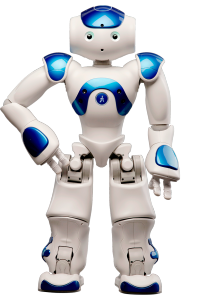
\includegraphics[width=0.8\textwidth]{Figures/NAO.png}
\\ ``Intelligence'' =
\end{minipage} 
\hfill{\scriptsize \cite{bachoptimization}}
\\
\hfill
\begin{minipage}[b]{0.2\textwidth}
\centering
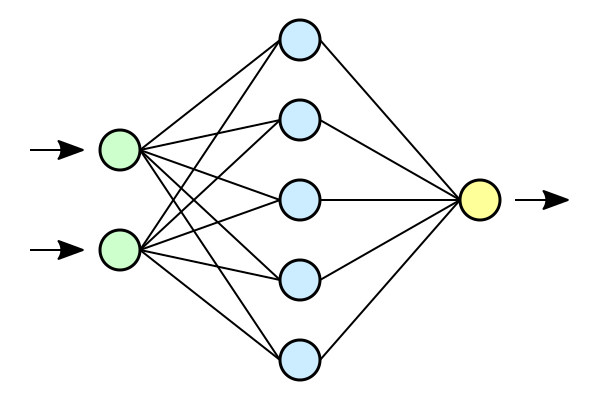
\includegraphics[width=\textwidth]{Figures/neural_network.png} \\
 models + 
\end{minipage} 
\begin{minipage}[b]{0.2\textwidth}
\centering
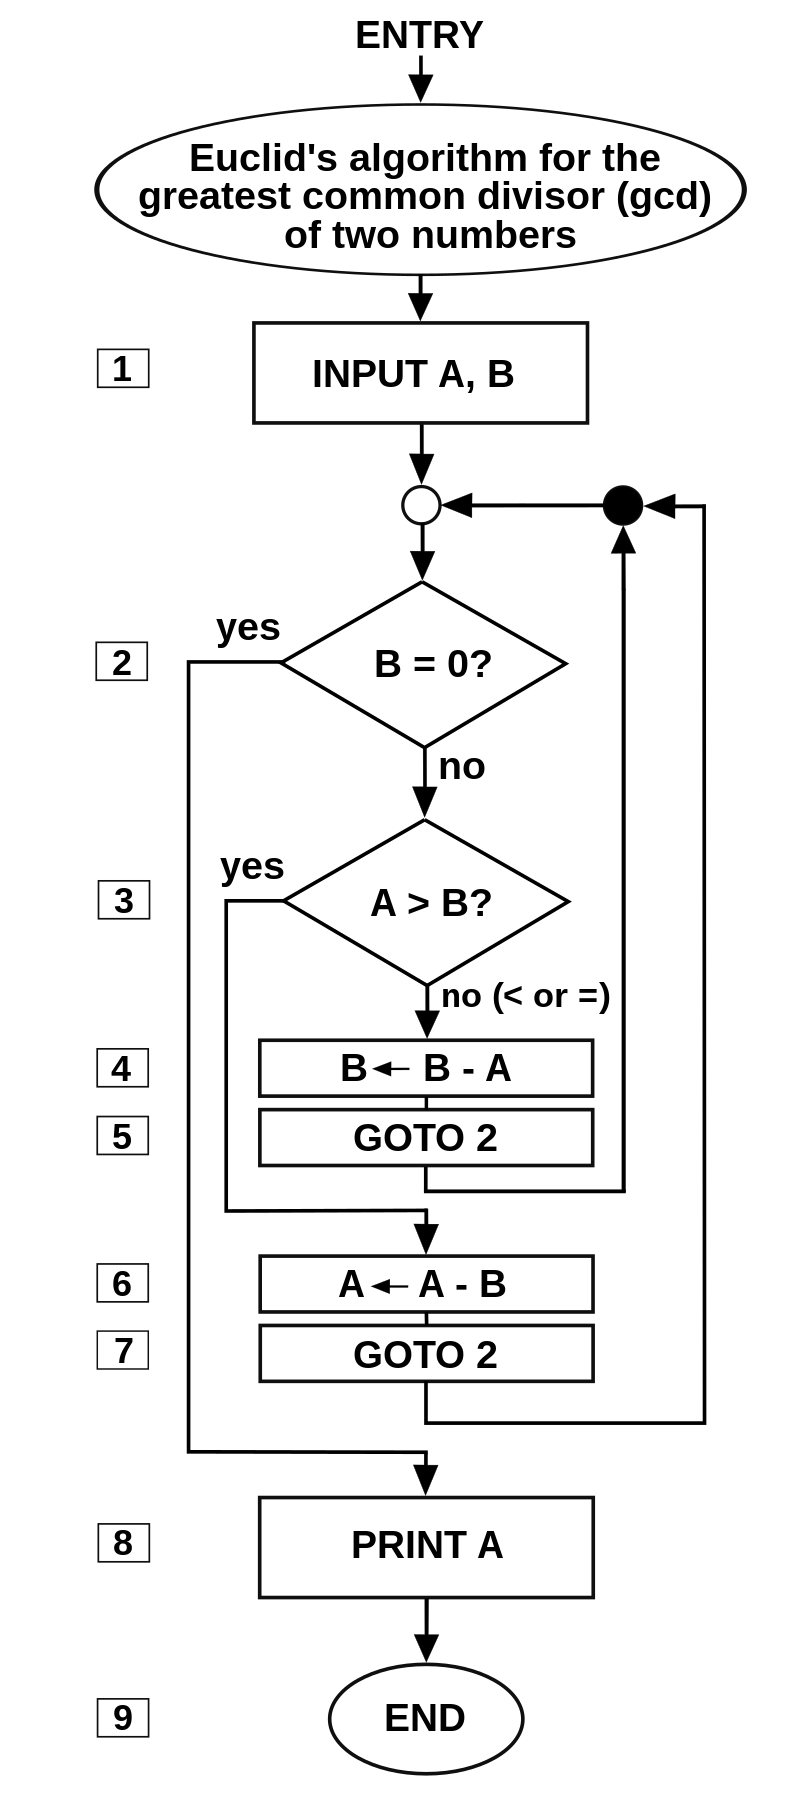
\includegraphics[width=0.5\textwidth]{Figures/algorithm.png} \\
\alert{algorithms} + 
\end{minipage} 
\begin{minipage}[b]{0.2\textwidth}
\centering
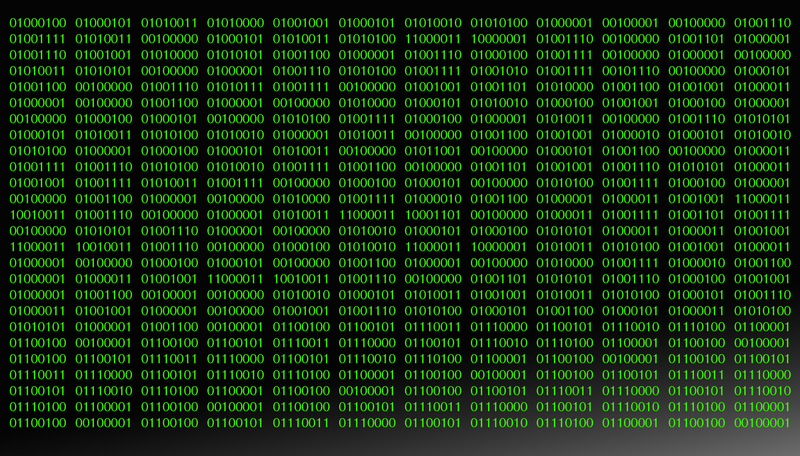
\includegraphics[width=\textwidth]{Figures/data.png} \\
data + 
\end{minipage} 
\begin{minipage}[b]{0.2\textwidth}
\centering
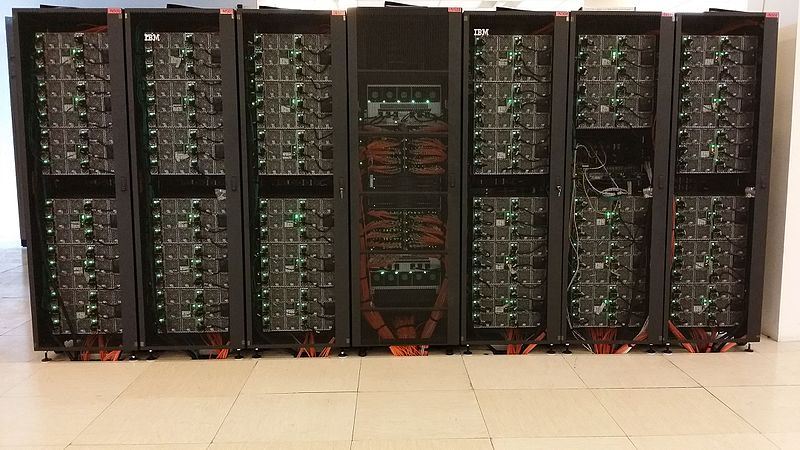
\includegraphics[width=\textwidth]{Figures/supercomputer.jpg} \\
computing power 
\end{minipage} 
%``Intelligence'' = models + \alert{algorithms} + data + computing power 
\end{frame}
\fi

%=======================================================================================
\begin{frame}
\frametitle{The advent of optimization algorithms}
\begin{minipage}[b]{0.25\textwidth}
\centering
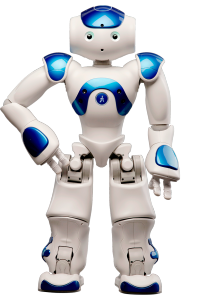
\includegraphics[width=0.8\textwidth]{Figures/NAO.png}
\\ ``Intelligence'' =
\end{minipage} 
\hfill
\begin{minipage}[b]{0.2\textwidth}
{\scriptsize \cite{bachoptimization}}
\vskip 3cm
~
\end{minipage} 
\\
\hfill
\begin{minipage}[t]{0.2\textwidth}
\centering
 models + 
\\
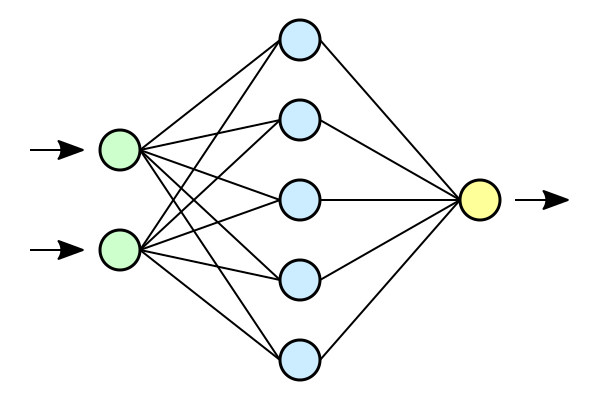
\includegraphics[width=\textwidth]{Figures/neural_network.png} 
\end{minipage} 
\begin{minipage}[t]{0.2\textwidth}
\centering
\textbf{\textcolor{red}{algorithms}} + 
\\
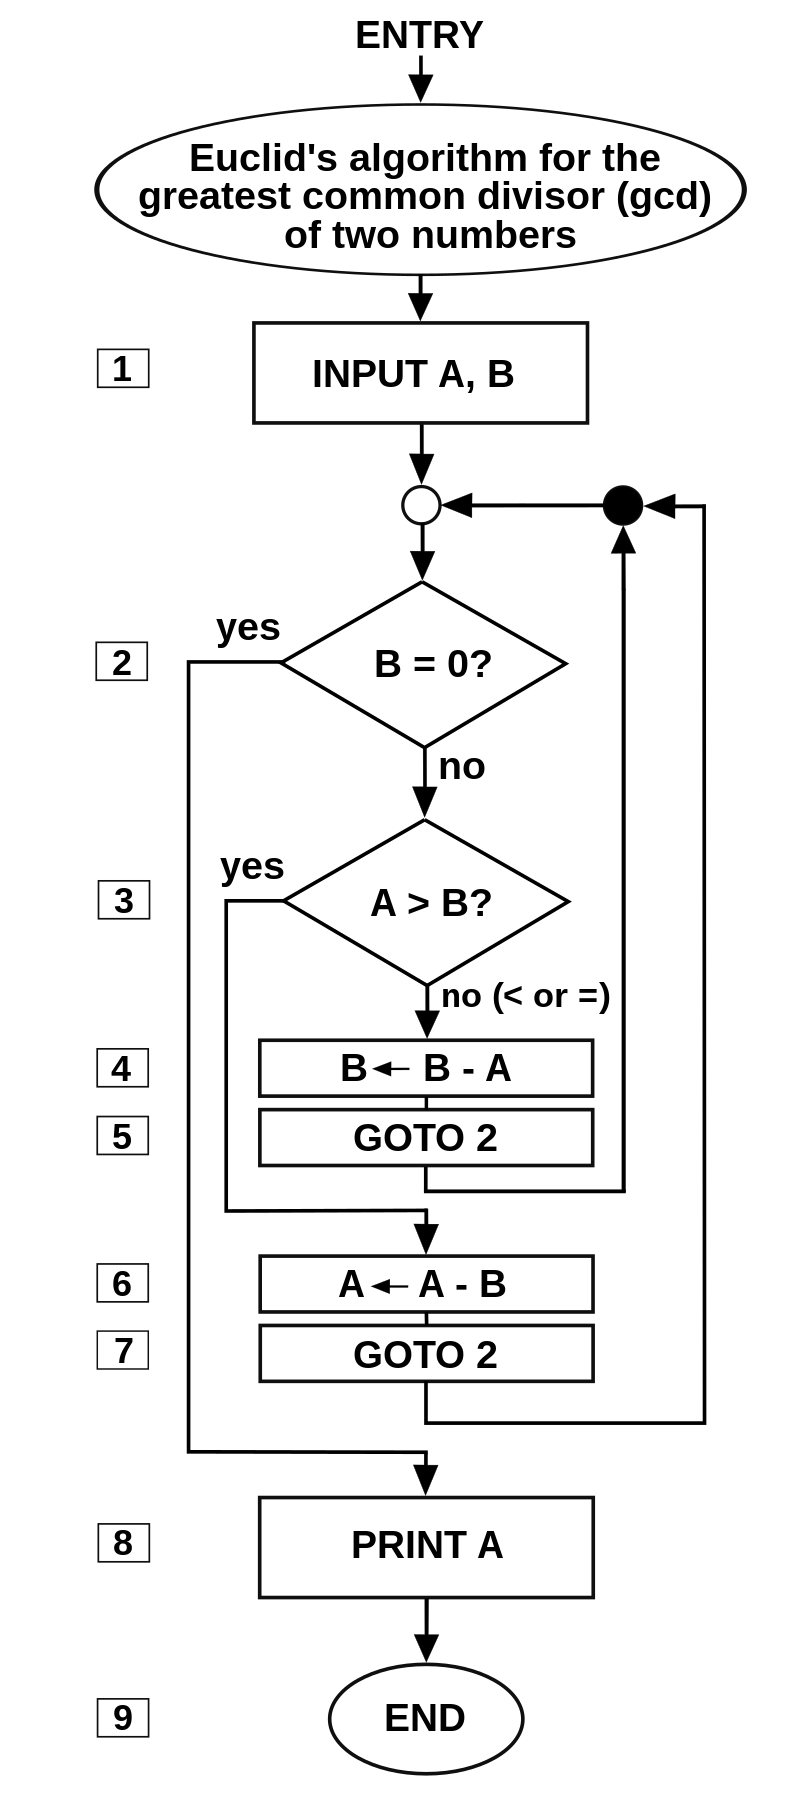
\includegraphics[width=0.5\textwidth]{Figures/algorithm.png} 
\end{minipage} 
\begin{minipage}[t]{0.2\textwidth}
\centering
data + 
\\\vskip 0.2cm
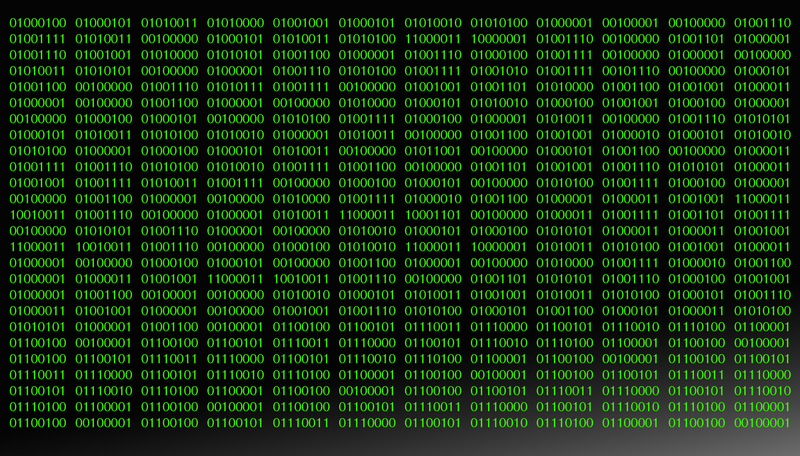
\includegraphics[width=\textwidth]{Figures/data.png} 
\end{minipage} 
\begin{minipage}[t]{0.2\textwidth}
\centering
computing power 
\\\vskip 0.2cm
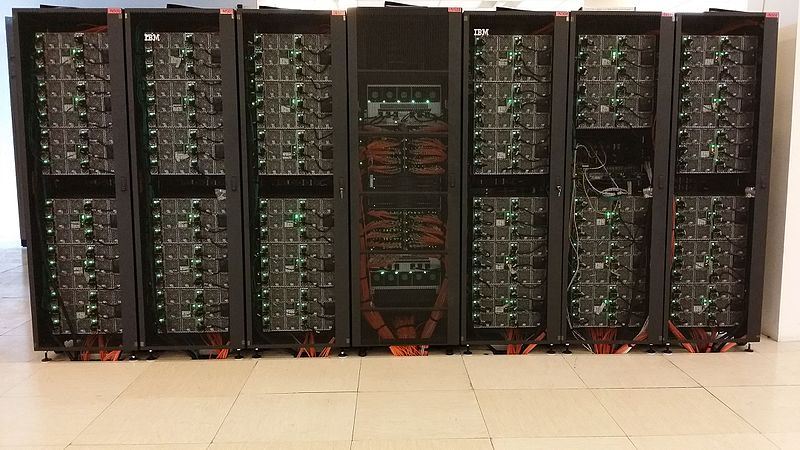
\includegraphics[width=\textwidth]{Figures/supercomputer.jpg} 
\end{minipage} 
%``Intelligence'' = models + \alert{algorithms} + data + computing power 
\end{frame}



\section{Bibliography}

%=======================================================================================
\begin{frame}[allowframebreaks]
\frametitle{References}
\scriptsize
%\vspace{-1.cm}
%\setbeamertemplate{bibliography item}{[\theenumiv]} % to have numbers in biblio with beamer
%   \bibliographystyle{plain}
   \bibliographystyle{apalike}
   \bibliography{biblio}
\end{frame}

\end{document}

